% =====================================================================
\section{Gradient Fields}\label{ch:gradfields}
% =====================================================================

\begin{definition}[Gradient vector field; Slides, Definition 3]\label{def:gradfield}
If $f$ is a scalar function of two variables, its gradient
\[
  \grad f(x,y)=\ip{f_x(x,y),\,f_y(x,y)}
\]
is a vector field on $\R^2$, called a \emph{gradient vector field}. Likewise, if
$f$ is a scalar function of three variables, its gradient
$\grad f(x,y,z)=\ip{f_x,\,f_y,\,f_z}$ is a vector field on $\R^3$.
\end{definition}

So every differentiable scalar function produces a vector field. By Lecture
Notes No.~6, the arrows of a gradient field (i) point in the direction of
fastest increase of $f$, (ii) have length equal to that fastest rate, and
(iii) are perpendicular to the level curves of $f$.

\begin{example}[Slides, Example 7.2]\label{ex:7.2}
Find the gradient vector field of $f(x,y)=x^2y-y^3$.
\end{example}
\begin{solution}
$f_x=2xy$ (treat $y$ as constant) and $f_y=x^2-3y^2$ (treat $x$ as constant). Hence
\[
  \grad f(x,y)=\ip{2xy,\;x^2-3y^2}=2xy\,\vi+(x^2-3y^2)\,\vj .
\]
Figure~\ref{fig:gradfield} draws this field on top of the level curves of $f$
(see also the Desmos graph linked on the slide). Every arrow crosses the level
curves at a right angle and points toward larger values of $f$; arrows are long
where the level curves are crowded together. At the origin
$\grad f=\vzero$ (a saddle-like critical point; the level curve $f=0$ consists
of the three lines $y=0$ and $y=\pm x$).
\end{solution}

\begin{figure}[H]
  \centering
  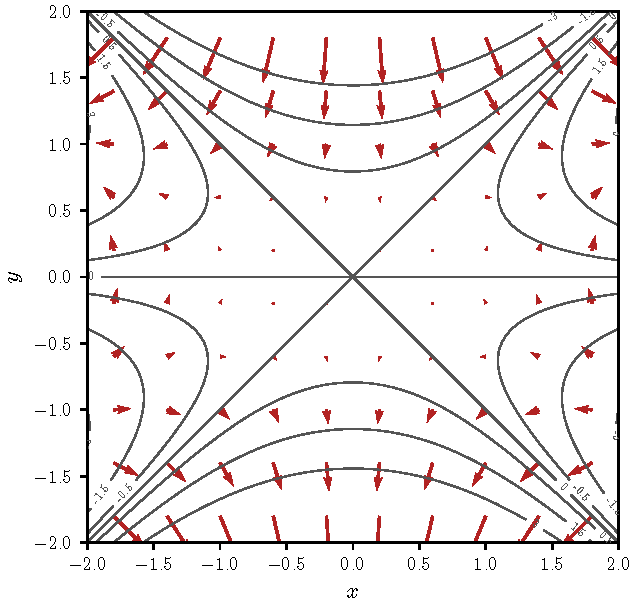
\includegraphics[width=0.55\linewidth]{gradient_field}
  \caption{Example 7.2: the gradient field $\grad f=\ip{2xy,x^2-3y^2}$ (red,
  scaled) over level curves of $f=x^2y-y^3$ (grey). Gradient vectors are
  perpendicular to the level curves.}
  \label{fig:gradfield}
\end{figure}

\begin{example}\label{ex:gradfield3}
Find the gradient field of (a) $f(x,y,z)=\frac12\ln(x^2+y^2+z^2)$ and
(b) $g(x,y,z)=\dfrac{c}{\sqrt{x^2+y^2+z^2}}$, $c$ a constant, and describe them.
\end{example}
\begin{solution}
Let $r=\norm{\vx}=\sqrt{x^2+y^2+z^2}$.

\textbf{(a)} By the chain rule,
$f_x=\frac12\cdot\frac{2x}{x^2+y^2+z^2}=\frac{x}{x^2+y^2+z^2}$, and similarly for $y,z$:
\[
  \grad f=\ip{\frac{x}{x^2+y^2+z^2},\,\frac{y}{x^2+y^2+z^2},\,\frac{z}{x^2+y^2+z^2}}=\frac{\vx}{r^2}.
\]
This is the field of Slides, Example~7.5: radial, pointing away from the
origin, with length $1/r$.

\textbf{(b)} Using $\grad(1/r)=-\vx/r^3$ (Lecture Notes No.~6, \S3.5, ``Gradient of
distance''), $\grad g=-c\,\vx/r^3$. With $c=mMG$ this is exactly the
gravitational field of Example~\ref{ex:gravity}. So gravity is a gradient field:
$\vF=\grad\!\left(\frac{mMG}{r}\right)$.
\end{solution}

\begin{example}\label{ex:gradfield-more}
Find the gradient fields of (a) $f=x^2+y^2$, (b) $f=e^x\cos y$,
(c) $f=xyz+z^2$.
\end{example}
\begin{solution}
\textbf{(a)} $\grad f=\ip{2x,2y}=2\vx$: radial outward, length $2r$.
\textbf{(b)} $\grad f=\ip{e^x\cos y,\,-e^x\sin y}$.
\textbf{(c)} $\grad f=\ip{yz,\;xz,\;xy+2z}$.
\end{solution}

\begin{remark}[The reverse question]
Computing $\grad f$ from $f$ is routine. The interesting question, and the
subject of the next chapter, is the \emph{reverse}: given a vector field $\vF$,
is it the gradient of some function, and if so, which one? For example, is
$\ip{yz,\,xz,\,xy+2z}$ a gradient? By (c) above, yes. Is $\ip{x^3y,\,xy}$? We
will see that it is not.
\end{remark}
